\documentclass{beamer}
\usepackage{beamerthemesplit}
\usepackage{graphics}
\logo{
\includegraphics[height=1cm]{psi_logo_white.png}}
\usetheme{Pittsburgh}
\usecolortheme{dove}
\beamertemplatenavigationsymbolsempty
\setbeamertemplate{footline}[frame number]
\definecolor{myback}{RGB}{175,238,238}
\setbeamercolor{structure}{bg=myback}
\usepackage[T1]{fontenc}
\newcommand{\changefont}[3] {
 \fontfamily{#1} \fontseries{#2} \fontshape{#3} \selectfont}

\title{NIAC Quo Vadis}
\author{Mark K\"onnecke }
\institute{NeXus International Advisory Committee}
\date{\today} 

\begin{document}

\begin{frame}
\titlepage
\end{frame}


\begin{frame}
\frametitle{The Future of NeXus }
\begin{itemize}
\item In existence since 1996
\item Uptake is very slooooooowwwwww
\item Things have changed since 1996
\item Do we leave NeXus as is?
\item Or do we change it based on our experiences, feedback?
\end{itemize}
\end{frame}


\begin{frame}
\frametitle{NeXus 2012}
\begin{itemize}
\item New things get done with NeXus
\item Problem: few new things get done
\item Problem: use of NeXus varies even across NeXus facilities
\item BUT: whenever other people try to devise a data format the 
 result looks much like NeXus: HDRI, tomography group, SAS
\end{itemize}
\end{frame}

\begin{frame}
\frametitle{Questionaire Feedback}
\begin{itemize}
\item From things said to us and the questionaire
\item We do not want NAPI: we want HDF-5
\item Too complicated
\begin{itemize}
\item NAPI
\item File hierarchy
\end{itemize}
\item Users do not see benefits
\item Bad documentation
\item Old formats as a barrier
\item Why change a running system?
\item Slow I/O
\item Lack of resources
\end{itemize}
\end{frame}


\begin{frame}
\frametitle{NeXus Usage}
\begin{itemize}
\item Soleil: 20 out of 26 instruments do NeXus, 2 Mill Files
\item PSI-SINQ: 11 from 16 instrument son NeXus, 1.4 Mill files
\item PSI-SLS: 0, 2 planned, 
\item SLS: none yet, planning to 
\item KEK: 10, 6 planned
\item ANSTO: 7 going to 10
\item ESRF: 2 beamlines, limited to NXentry, NXcollection, NXdata, moving to 4
\item HZB: 3N, 3 planned 
\item FRM 2: 0, moving to 1
\item SNS: 14,3 in the pipeline
\item DESY: 0, 11 in 2 Jahren
\item Diamond: 7 NeXus only, 17 writing, moving to 18 as primary format
\item ISIS: 8 using, 20 writing, planned: 20 using
\item Muons: 4 instruments, reluctance to move on
\item Lujan/LANL: 11 instruments, no change
\end{itemize}
\end{frame}

\begin{frame}
\frametitle{NIAC Tasks}
\begin{itemize}
\item Need to find something only NeXus can do
\item ESRF would like a simpler NeXus: NeXus ultralight or NXexchange
\item ESRF: NIAC as a custodian
\item Collect examples
\item Work better with SW groups at facilities in construction
\item Work for reduced data interchange
\item Provide NeXus tools as components to be integrated into other SW
\item Try to integrate stronger with communities
\end{itemize}
\end{frame}


\begin{frame} \frametitle{NeXus Energy Curve}
\begin{figure}[!ht]
\resizebox{8cm}{6cm}{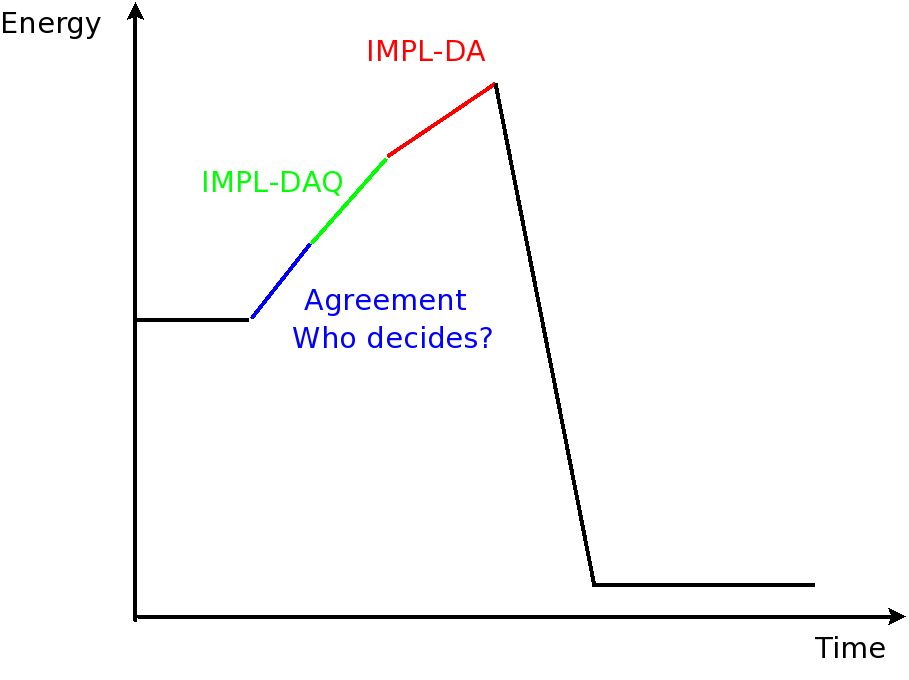
\includegraphics[width=0.9\textwidth]{dfenergy.png}}\end{figure}
\end{frame}

\begin{frame}
\frametitle{Reaching Agreement}
\begin{itemize}
\item No scientific body to decide upon data formats
\item Little interest from scientist in computing and data formats
\begin{itemize}
\item MUST produce papers, papers, papers....
\end{itemize}
\item Data format problems solved by computing slaves or PHD students
\begin{itemize}
\item People with little political clout in facility hacking order
\end{itemize}
\end{itemize}
\end{frame}


\begin{frame}
\frametitle{Data Ownership Issues}
\begin{itemize}
\item Producing facility generates and owns data
\begin{itemize}
\item May need to do non standard things in order to optimize writing
\item My define a facility standard format to save man power
\end{itemize}
\item Scientific communities own data analysis
\begin{itemize}
\item They decide what they need
\end{itemize}
\end{itemize}
\end{frame}


\begin{frame}
\frametitle{Implementation Issues}
\begin{itemize}
\item Facilities minimise computing resources 
\item Competition for scarce scientific computing resources
\item More sexy then data formats:
\begin{itemize}
\item Get that screwed instrument to work
\item Implement that new data analysis algorithm
\item Advice dumber and dumber users
\end{itemize}
\end{itemize}
\end{frame}

\begin{frame}
\frametitle{Conflicting Aims in NeXus}
\begin{itemize}
\item Full NeXus organises a complete beamline description with 
  possibly hundreds of parameters 
\begin{itemize}
\item Hierarchy a good thing
\end{itemize}
\item An application definition ownly contains less then 30 parameters
\begin{itemize}
\item Hierarchy looks like overkill
\end{itemize}
\item Features like workflow in file, multiple experiments rarely used
\end{itemize}
\end{frame}

\begin{frame}
\frametitle{Dictionary Based Programming Techniques}
\begin{itemize}
\item Soleil and ANSTO: Common Data Modell (CDM)
\end{itemize}
\begin{enumerate}
\item Use: H5Oopen(fid,''/entry/detector/data'',NULL,NULL)
\item Externalize path strings into separate files
\end{enumerate}
\begin{itemize}
\item Consequences:
\begin{itemize}
\item By editing dictionary any file containing the data can be read
\item Fixed paths and names no longer important
\end{itemize}
\end{itemize}
\end{frame}

\begin{frame}
\frametitle{Tree Based Programming}
\begin{itemize}
\item Read in whole file hierarchy
\item On demand loading for large arrays
\item Then pick your data nuts and raisins from the tree
\end{itemize}
\end{frame}

\begin{frame}
\frametitle{Are Data Format Requirements Changing?}
\begin{itemize}
\item 1996, diskspace expensive: snapshot of instrument was what was possible
\item 2012, diskspace shit cheap:
\begin{itemize}
\item Event mode for neutrons
\item On the fly scans at synchrotrons
\item FELS experiments log only
\item Full logging of experiment becomes possible (and desirable)
\end{itemize}
\item Demand for more time stamped data
\item Data files would be extracted from logs as interface to legacy DA software
\end{itemize}
\end{frame}



\begin{frame}
\frametitle{Value in NeXus}
\begin{itemize}
\item The dictionary of names and terms
\begin{itemize}
\item Needs better documentation and definition though
\item It does not matter where things are in the file but meaning is 
 still important
\end{itemize}
\item Application definitions as starting points for method specific standards
\item Standard validation tools
\item NeXus Rules
\begin{itemize}
\item Scan storage rules
\item Axis assignment rules
\item Coordinate system rules
\end{itemize}
\end{itemize}
\end{frame}

\begin{frame}
\frametitle{NeXus Options}
\begin{itemize}
\item Hold on tight!
\item Simplified NeXus
\item NIAC as a custodian
\item Give up
\item Your option here
\end{itemize}
\end{frame}


\begin{frame}
\frametitle{Simplified NeXus}
\begin{itemize}
\item Make hierarchy a recommendation
\item Ultralight:
\begin{itemize}
\item Use HDF-5
\item Use dictionary based programming
\end{itemize}
\item Light:
\begin{itemize}
\item Use NXentry and NXsubentry
\item Possibly flatten NXsubentry hierarchy
\item Collect data items for exchange
\end{itemize}
\item Medium:
\begin{itemize}
\item Flatten NXinstrument
\item Limit us to one way to define orientation and position of components
\end{itemize}
\end{itemize}
\end{frame}

\begin{frame}
\frametitle{NIAC as Custodian}
\begin{itemize}
\item NIAC as forum for discussing data formats
\item NIAC stores, documents and maintains community developed formats
\item NIAC maintains NeXus dictionaries
\end{itemize}
\end{frame}


\begin{frame}
\frametitle{Questions to be answered}
\begin{itemize}
\item Where do we want to go with NeXus?
\item Do we reinvent NeXus?
\item Do we provide more for time stamped data?
\item Which role do you envisage for the NIAC?
\item Do we invest in OO-NeXus?
\item What do we do with NAPI?
\item Opinions???
\end{itemize}
\end{frame}






\end{document}


\begin{frame}
\frametitle{}
\begin{itemize}
\item
\item
\item
\item
\end{itemize}
\end{frame}
